\chapter{Consideraciones finales y conclusiones}
\label{conclusiones}

A lo largo del trabajo se han realizado varias reconstrucciones tomográficas de distintos
objetos, para verificar visualmente la efectividad de la alineación en situaciones reales.

\section{Algunas reconstrucciones tomográficas}

Las siguientes son imágenes obtenidas a partir de reconstrucciones tomográficas, adquiridas con
el microtomógrafo. La figura \ref{fig:reloj_rec} presenta dos cortes tomográficos del mecanismo
de un reloj reconstruidos a partir de una misma adquisición (mismos parámetros). Sin embargo, se utilizaron distintos
parámetros en la reconstrucción, alineados en una y desalineados en la otra, diferencia que se
observa claramente por los artefactos de ``doble imagen'' en la fig. \ref{fig:reloj_rec}.b. Esto
demuestra la importancia de la correcta alineación y calibración geométrica, incluso si las
correcciones parecen ``pequeñas''. La figura \ref{fig:reloj3d} es la reconstrucción tridimensional
correspondiente a la fig. \ref{fig:reloj_rec}.a, y se observa una muy buena definición de las
formas geométricas y volúmenes de las piezas mecánicas. Algunas partes parecen más ``difuminadas'',
a causa de ser componentes con superficie amplia pero muy delgados.

Por otro lado, en las figuras \ref{fig:hueso_rec} y \ref{fig:vertebra_rec} se observan reconstrucciones
de muestras biológicas, con formas orgánicas y no tan definidas como las piezas mecánicas de un
reloj. Aún así, se observa un alto nivel de detalle, y se se llegan a apreciar características de
las muestras (como cavidades) de tamaños de hasta 50 $\mu$m. En la figura \ref{fig:hueso_rec}.b
parece haber artefactos de líneas rectas, sobre todo en las zonas más densas del hueso, causadas
por el ``re-slicing'' que se hizo a partir de los cortes transversales de \ref{fig:hueso_rec}.a.
Sin embargo, no parece haber otros artefactos. La figura \ref{fig:vertebra_rec} por otro lado,
aunque también presenta una muy buena resolución espacial, parece tener más artefactos de intensidad,
como puntos y líneas más brillantes, o un ``ruido'' alrededor de la vértebra, debido a la presencia
de elementos de alta densidad en ciertas regiones.

Finalmente, la figura \ref{fig:mandibulas} muestra dos cortes transversales de mandíbulas de rata (muestras distintas, pero comparables),
reconstruidos a partir de una reconstrucción con un microtomógrafo Bruker y con el de arquitectura
abierta, y adquiridas con los mismos parámetros. Aunque los cortes no son de la misma muestra, se observa que en cuestión
de calidad de imagen, nivel de detalle, reconstrucción de las formas y resolución espacial, ambas
reconstrucciones son comparables, y prácticamente imposible de determinar el origen de cada una.

\begin{figure}[htpb]
    \centering
    \begin{subfigure}{0.49\textwidth}
        \begin{overpic}[width=\linewidth]{images/reloj_rec.png}
            \put(3, 90){\colorbox{black!60}{\color{white}\bfseries\large (a)}}
        \end{overpic}
    \end{subfigure}
    \hfill
    \begin{subfigure}{0.49\textwidth}
        \begin{overpic}[width=\linewidth]{images/reloj_rec1.png}
            \put(3, 90){\colorbox{black!60}{\color{white}\bfseries\large (b)}}
        \end{overpic}
    \end{subfigure}
    \caption{Cortes tomográficos reconstruidos del mecanismo de un reloj, a partir de parámetros corregidos
    (\textbf{a}) y a partir de un sistema desalineado (\textbf{b}). En la segunda, se observa una
    ``superposición'' de imágenes, con una leve diferencia angular, causada por la desalineación. Parámetros
    de adquisición: 90 kV (Voltaje), 47 $\mu$A (Corriente), 1200 proyecciones, $M=2.55$ y resolución de pixel
    de 24.4 $\mu$m.}
    \label{fig:reloj_rec}    
\end{figure}

\begin{figure}[htpb]
    \centering
    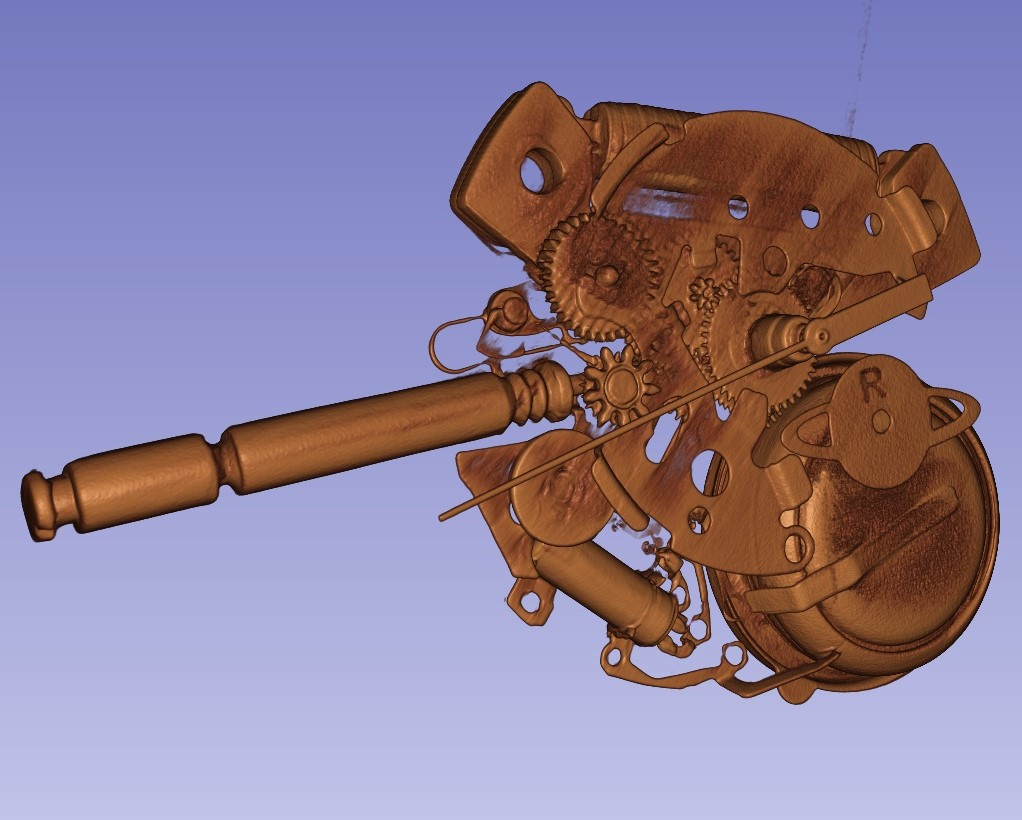
\includegraphics[width=0.65\textwidth]{images/reloj3d.jpg}
    \caption{Visión tridimensional de la reconstrucción tomográfica del mecanismo de un reloj
    (utilizando el software 3DSlicer).}
    \label{fig:reloj3d}
\end{figure}

\begin{figure}[htpb]
    \centering
    \begin{subfigure}{0.26\textwidth}
        \begin{overpic}[width=\linewidth]{images/hueso_rec1.png}
            \put(1, 88){\colorbox{black!60}{\color{white}\bfseries\large (a)}}
        \end{overpic}
    \end{subfigure}
    \hfill
    \begin{subfigure}{0.73\textwidth}
        \begin{overpic}[width=\linewidth]{images/hueso_rec2.png}
            \put(0.5, 31.5){\colorbox{black!60}{\color{white}\bfseries\large (b)}}
        \end{overpic}
    \end{subfigure}
    \caption{Reconstrucción tomográfica de un hueso (fémur) de rata. \textbf{a)} Corte tomográfico
    axial, donde se pueden observar cavidades de hasta 50 $\mu$m de diámetro. \textbf{b)} Corte
    tomográfico sagital (rotado 90$^{\circ}$) del hueso. Se observan diferencias de densidad en distintas
    regiones del hueso, dadas por las diferencias de intensidad. Parámetros de adqusición: 90 kV (voltaje),
    47 $\mu$A (corriente), 1200 proyecciones, $M=2.06$ y resolución de pixel de 24.3 $\mu$m.}
    \label{fig:hueso_rec}    
\end{figure}

\begin{figure}[htpb]
    \centering
    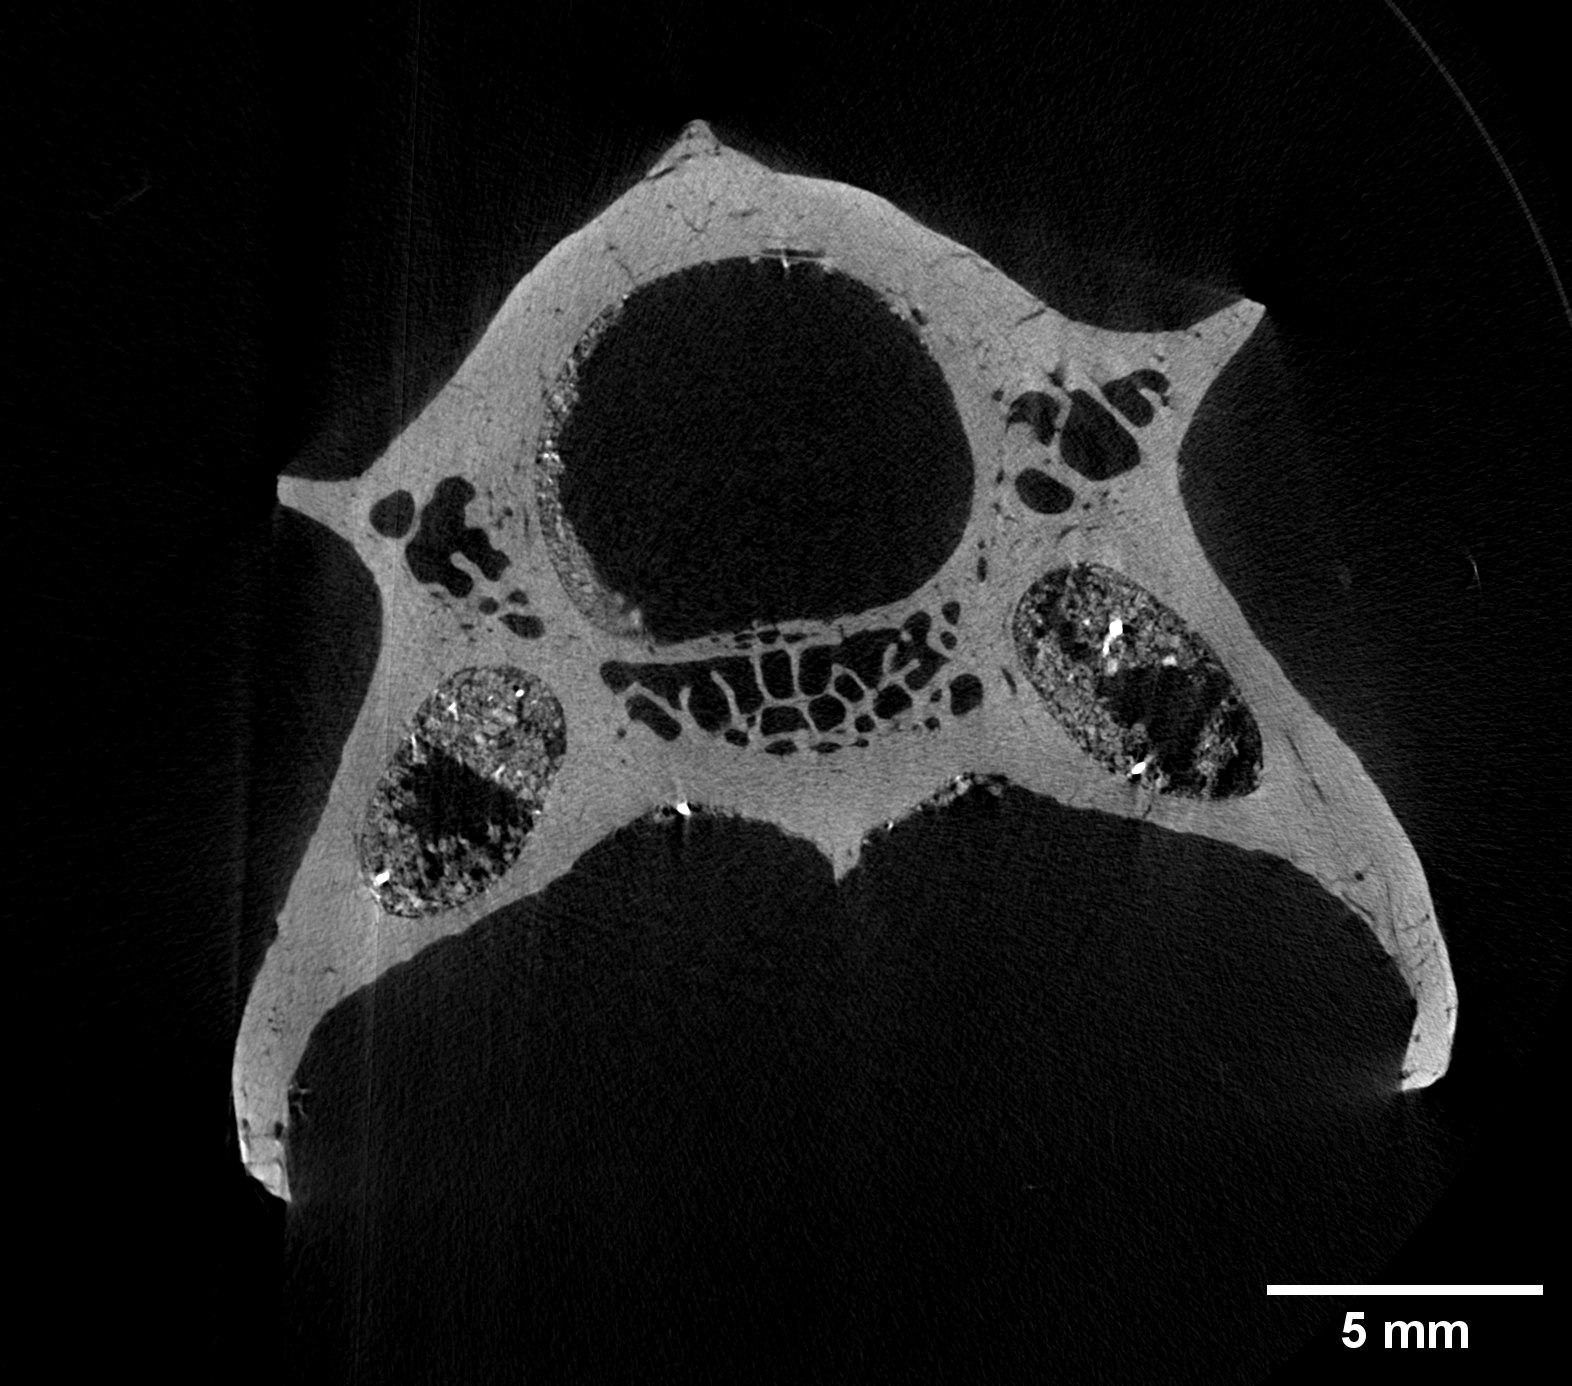
\includegraphics[width=0.5\textwidth]{images/verte_rec_0.png}
    \caption{Corte tomográfico axial reconstruido de una vértebra, correspondiente a las proyecciones
    de la figura \ref{fig:vertebra}.}
    \label{fig:vertebra_rec}
\end{figure}

\begin{figure}[htpb]
    \centering
    \begin{subfigure}{0.40\textwidth}
        \begin{overpic}[width=\linewidth]{images/mandibula_BK.png}
            \put(3, 90){\colorbox{black!60}{\color{white}\bfseries\large (a)}}
        \end{overpic}
    \end{subfigure}
    \hspace{7mm}
    \begin{subfigure}{0.40\textwidth}
        \begin{overpic}[width=\linewidth]{images/mandibula_AA.png}
            \put(3, 90){\colorbox{black!60}{\color{white}\bfseries\large (b)}}
        \end{overpic}
    \end{subfigure}
    \caption{Cortes transversales reconstruidos de dos mandíbulas de rata similares. (\textbf{a})
    Reconstrucción a partir de una adquisición con un microtomógrafo marca Bruker. (\textbf{b})
    Reconstrucción a partir de una adquisición con el microtomógrafo de arquitectura abierta
    trabajado. Parámetros de adquisición: 70 kV (Voltaje), 142 $\mu$A (Corriente), 471 proyecciones,
    $M=1.44$, resolución de pixel de 25.0 $\mu$m.}
    \label{fig:mandibulas}    
\end{figure}

\newpage

\section{Conclusiones}

A partir del desarrollo experimental y el análisis de resultados presentados en este trabajo,
se pueden extraer las siguientes conclusiones generales en relación con los objetivos planteados
inicialmente:

Se cumplió satisfactoriamente con la optimización
del microtomógrafo de arquitectura abierta del laboratorio LAMARX. La transición hacia un
diseño con fuente y detector fijados sobre una base rígida fue un paso crítico que permitió
minimizar las desalineaciones accidentales y garantizó la estabilidad necesaria para procesos
de adquisición prolongados.

La alineación física inicial, mediante el análisis de círculos proyectados y la
superposición de cilindros reflejados, demostró ser un método robusto para reducir las
desviaciones angulares fuera de plano ($\theta$ y $\phi$) a valores menores a 5$^{\circ}$, y para
aproximar el punto principal del eje de magnificación al centro del detector. No
obstante, se concluye que este proceso tiene una alta dependencia de la destreza del
operador y de particularidades mecánicas del sistema.

En cuanto a la calibración analítica, el método de múltiples proyecciones y análisis de trayectorias
elípticas resultó
ser una herramienta altamente confiable y consistente para determinar parámetros finos como
la distancia fuente-detector $D$, la distancia fuente-objeto $F$, la posición del punto principal $\mathcal{P}$,
y la inclinación de los ejes en el plano del detector ($\eta$).
Por el contrario, el método de una única proyección se reveló
como inconsistente e impráctico para las condiciones del laboratorio, debido a su extrema
sensibilidad a la posición del fantoma y a la amplificación de errores en sus
complejas operaciones matemáticas.

Se logró caracterizar eficazmente la resolución espacial del sistema a partir del análisis de
la función de transferencia de modulación ($MTF$), obtenida del análisis de bordes. Se determinó
que para este sistema, se tiene una resolución espacial de entre 15 y 60
$\mu$m, en el rango de magnificaciones posibles del detector ($M<7$). Se concluye que las aproximaciones
teóricas estándar de la resolución subestiman este valor, lo que validó la necesidad de introducir una
corrección empírica (parámetro $c$) para modelar adecuadamente el comportamiento del equipo.
Asimismo, se verificó que el método de la lámina inclinada es un sustituto rápido y equivalente
a la medición sobre reconstrucciones tomográficas para caracterizar la MTF.

La implementación manual de técnicas de
pre-procesamiento fue determinante para la calidad de los resultados finales. La Corrección
de Campo Plano (FFC) no solo uniformizó la intensidad del haz, sino que eliminó con éxito el
patrón hexagonal del detector y las estructuras electrónicas de ruido, logrando aumentar la
relación señal-ruido (SNR) en un factor de 2.4. Adicionalmente, la corrección temporal compensó
eficazmente la inestabilidad de la fuente de rayos X, asegurando una reconstrucción libre
de artefactos de intensidad.

La efectividad de todo el protocolo desarrollado
fue validada visualmente mediante la reconstrucción de objetos complejos. La obtención de
imágenes nítidas en muestras biológicas (fémur de rata, mandíbula y vértebra) y mecánicas, con la
capacidad de distinguir microestructuras (del tamaño esperado según los cálculos de resolución
espacial), confirma que el sistema se encuentra
calibrado para realizar investigación científica de alta precisión, compitiendo con un
microtomógrafo comercial de alto nivel. A su vez, se probó la
repetibilidad del protocolo, al ser utilizado más de una vez, en configuraciones distintas del
sistema.

En conclusión, este trabajo establece un protocolo de calibración sistemático y reproducible,
transformando un conjunto de componentes independientes en un instrumento de microtomografía
funcional y preciso, capaz de competir con soluciones comerciales en términos de calidad de imagen,
flexibilidad y trazabilidad de datos.

\subsection{Perspectivas a futuro}

La naturaleza de ``arquitectura abierta'' del microtomógrafo implica un potencial inmenso de
mejoras y modificaciones, todas en función del tipo de uso que se requiera del mismo.

En primer lugar, y continuando con las ideas presentadas en el capítulo \ref{cap:cal_intensidad},
es de interés diseñar un método de calibración del nivel de gris, para lograr mediciones reales
y consistentes del coeficiente de atenuación lineal de una muestra, utilizando materiales de
referencia o nuevos fantomas.

Por otro lado, se puede seguir avanzando sobre la estructura física del mismo. Algunas ideas
ya se han nombrado a lo largo del trabajo, como mejorar la base de soporte y el sistema de rieles, acoplar
el porta-muestra a esta misma base (y tener un sistema totalmente acoplado), mejorar los sistemas de
fijación de las muestras, añadir más micro-motores,
y por lo tanto, grados de libertad de movimiento controlado a cada componente, entre otros.

También sería posible realizar avances en el software del equipo, ya sea para añadir otros componentes
como micro-motores, o para el procesamiento y análisis de las proyecciones radiográficas y tomografías.
En este trabajo, se demostró la utilidad de herramientas como FIJI, capaces de implementar macros y
plugins que automatizan procesos complejos, pero solo se observó una pequeña fracción de su potencial.
Por otro lado, la corrección de algunos artefactos, como el endurecimiento del haz, son posibles de tratar
solamente con softwares especializados.

En este campo y por último, es importante destacar el gran avance
que han tenido los modelos de Machine Learning y Redes Neuronales para el tratamiento de imágenes,
no solo en la identificación y corrección de errores y artefactos, sino también en la
segmentación avanzada y automatizada. 
